\documentclass[aps,nofootinbib,onecolumn,groupedaddress,a4paper]{revtex4}

\usepackage{color}
\usepackage{graphicx}
\usepackage[utf8]{inputenc}

\usepackage{listings}

\lstset{
  language=Python,
  showstringspaces=false,
  formfeed=\newpage,
  tabsize=4,
  commentstyle=\itshape,
  basicstyle=\ttfamily,
  morekeywords={models, lambda, forms}
}


\begin{document}

\title{Photoelectric Effect} 

\author{Adnan Basar}
\affiliation{Phys 442.01\\
2010205108}


\date{March 09, 2013}

\begin{abstract}
The objective of this experiment is to demonstrate the quantization of energy in electromagnetic
waves and to determine Planck's constant $h$.
\end{abstract}

\maketitle


\section{Introduction}
It was discovered by Heinrich Hertz that light incident
upon a matter target caused the emission of electrons
from the target.The effect was termed the Hertz Effect
(and later the Photoelectric Effect) and the electrons referred to as photo electrons. It was understood that the
electrons were able to absorb the energy of the incident
light and escape from the coulomb potential that bound
it to the nucleus.\\

According to classical wave theory, the energy of a
light wave is proportional to the intensity of the light
beam only. Therefore, varying the frequency of the light
should have no effect on the number and energy of resultant photoelectrons. We hope to disprove this classical hypothesis through experimentation, by demonstrating that the energy of light does indeed depend on the frequency of light, and that this dependence is linear with Planck’s constant h as the constant of proportionality.\\

Light comes in discrete packets, called photons, each
with an energy proportional to its frequency.
\begin{center}
$E=h\upsilon$
\end{center}

For each metal, there exists a minimum binding energy
for an electron characteristic of the element, also called
the work function (${W}_{0}$). When a photon strikes a bound
electron, it transfers its energy to the electron. If this
energy is less than the metal’s work function, the photon
is re-emitted and no electrons are liberated. If this energy
is greater than an electron’s binding energy, the electron
escapes from the metal with a kinetic energy equal to
the difference between the photon’s original energy and
the electron’s binding energy (by conservation of energy).
Therefore, the maximum kinetic energy of any liberated
electron is equal to the energy of the photon less the
minimum binding energy (the work function). Expressed
concisely the relationship is as such:
\begin{center}
${K}_{max}=h\upsilon-{W}_{0}$
\end{center}

When $e{V}{s} = {K}_{max}$ we will cease to see any current
through the circuit. By finding this voltage we calculate
the maximum kinetic energy of the electrons emitted as a
function of radiation frequency.


\section{Experimental Setup}
\begin{itemize}
\item High pressure mercury lamp with power supply
\item Spectrograph with a transmission grating
\item Photocell with housing
\item Current Amplifier
\item Moving coil DC Voltmeter for the current amplifier (0-3 V)
\item DC Voltmeter (0-3 V)
\item Connecting leads
\item Power supply (0-3 V)
\end{itemize}


\section{Data and Analysis}

Our experiment has some data for each color:\\


\begin{table}
\caption{Yellow \label{rawdata}}
\centering
\begin{tabular}{ccc}
\\
$Current$ $(A {10}^{-10})$ & $Volatge$ $(V)$ \\
\hline
-0.06 		&  0.800  	\\
-0.05    	&  0.745  	\\
-0.01 		&  0.460 	\\
0 			&  0.405  	\\
0.1 		&  0.256  	\\
0.2 		&  0.167   	\\
0.3 		&  0.105   
\end{tabular}
\label{default}
\end{table}

\begin{table}
\caption{Green \label{rawdata}}
\centering
\begin{tabular}{ccc}
\\
$Current$ $(A {10}^{-10})$ & $Volatge$ $(V)$ \\
\hline
-0.12 &  1.705   \\
-0.10 &  0.977  \\
-0.05 &  0.565  \\
0 & 0.491  \\
0.10 & 0.405  \\
0.15 & 0.374   \\
0.30 & 0.298   
\end{tabular}
\label{default}
\end{table}%

\begin{table}
\caption{Turquoise \label{rawdata}}
\centering
\begin{tabular}{ccc}
\\
$Current$ $(A {10}^{-10})$ & $Volatge$ $(V)$ \\
\hline
-0.02 &  2.129   \\
-0.015 &  1.292  \\
-0.010 &  0.908 \\
0 & 0.594  \\
0.05 & 0.367  \\
0.10 & 0.237   \\
0.15 & 0.095   
\end{tabular}
\label{default}
\end{table}%

\begin{table}
\caption{Blue \label{rawdata}}
\centering
\begin{tabular}{ccc}
\\
$Current$ $(A {10}^{-10})$ & $Volatge$ $(V)$ \\
\hline
-0.15 &  1.961   \\
-0.10 &  1.268  \\
-0.05 &  1.103  \\
0 &      1.008  \\
0.05 &   0.968  \\
0.10 &   0.925   \\
0.20 &   0.859   
\end{tabular}
\label{default}
\end{table}

\begin{table}
\caption{Violet \label{rawdata}}
\centering
\begin{tabular}{ccc}
\\
$Current$ $(A {10}^{-10})$ & $Volatge$ $(V)$ \\
\hline
-0.05 &  1.495   \\
-0.02 &  1.281  \\
-0.01 &  1.220  \\
0 &      1.119\\
0.05 &   1.022  \\
0.10 &   0.920   \\
0.20 &   0.811   
\end{tabular}
\label{default}
\end{table}

I used ${V}_{s}$ error as 0.02 V in finding stopping voltage is fitted graphs. \\

\begin{figure}[h]
\caption{Yellow \label{rawplot}}
\includegraphics[width=1.0 \columnwidth]{yellow.eps}
\end{figure}

\begin{figure}[h]
\caption{Green \label{rawplot}}
\includegraphics[width=1.0 \columnwidth]{green.eps}
\end{figure}

\begin{figure}[h]
\caption{Turquoise \label{rawplot}}
\includegraphics[width=1.0 \columnwidth]{turq.eps}
\end{figure}

\begin{figure}[h]
\caption{Blue \label{rawplot}}
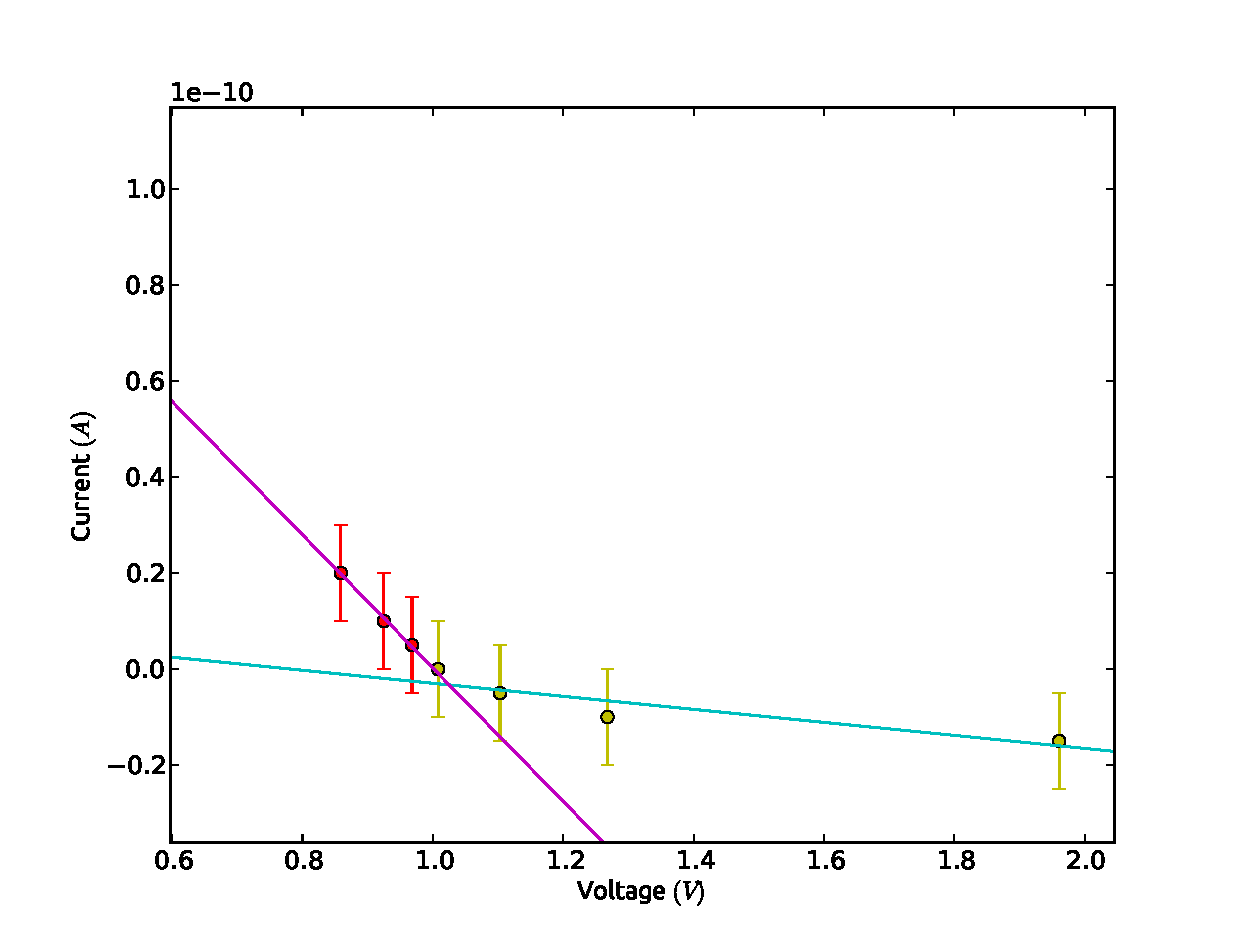
\includegraphics[width=1.0 \columnwidth]{blue.eps}
\end{figure}

\begin{figure}[h]
\caption{Violet \label{rawplot}}
\includegraphics[width=1.0 \columnwidth]{mor.eps}
\end{figure}

Any linear regression $y = mx + b$ calculated from our
input variables and errors outputs an uncertainty on m
and on $b$. In the case of finding the intersection of two
linear regression lines $y = m_{1}x+b_{1}$ and $y = m_{2}x+b_{2}$, the
error propagation formula was used to derive the following result for error on the X-coordinate of the intersection point in 2-D space:

\begin{center}


$\sigma_x^2 = \left(\frac{1}{m_1 - m_2}\right)^2 \sigma_{b_2}^2 + 
             \left(\frac{1}{m_1 - m_2}\right)^2 \sigma_{b_1}^2 +
		 \left(\frac{b_2 - b_1}{(m_1 - m_2)^2}\right)^2 \sigma_{m_1}^2 +
		 \left(\frac{b_2 - b_1}{(m_1 - m_2)^2}\right)^2 \sigma_{m_2}^2$
\end{center} 

From these way I found :

\begin{table}[ht]
\caption{Voltage Stopping \label{rawdata}}
\centering
\begin{tabular}{cccccc}
\\
& Yellow & Green & Turquoise & Blue & Violet  \\
\hline
$V_s (V)$& 0.329 &  0.471 &0.596 & 1.025 & 1.069 \\

$\sigma V_s(V)$ &0.020 & 0.026 & 0.053 & 0.096 & 0.150 \\

$\upsilon ({10}^{14}Hz)$ & 5.19 & 5.49 & 6.08 & 6.88 & 7.41 


  
\end{tabular}
\label{default}
\end{table}

By Using Table VI values, I fitted values to estimate $h$ and ${W}_{0}$ with errors in such $y=max+n$

\begin{center}
$V_s=\frac{h}{q}\upsilon-\frac{1}{q}W_0$

\end{center}

where $h=1.6x10^{-19}  m $, $\sigma_h=1.6x10^{-19}\sigma_m$,$W_0=-n$ and $\sigma_{W_0}=\sigma_n$\\.

\begin{figure}[h]
\caption{ Planck's Constant Estimation \label{rawplot}}
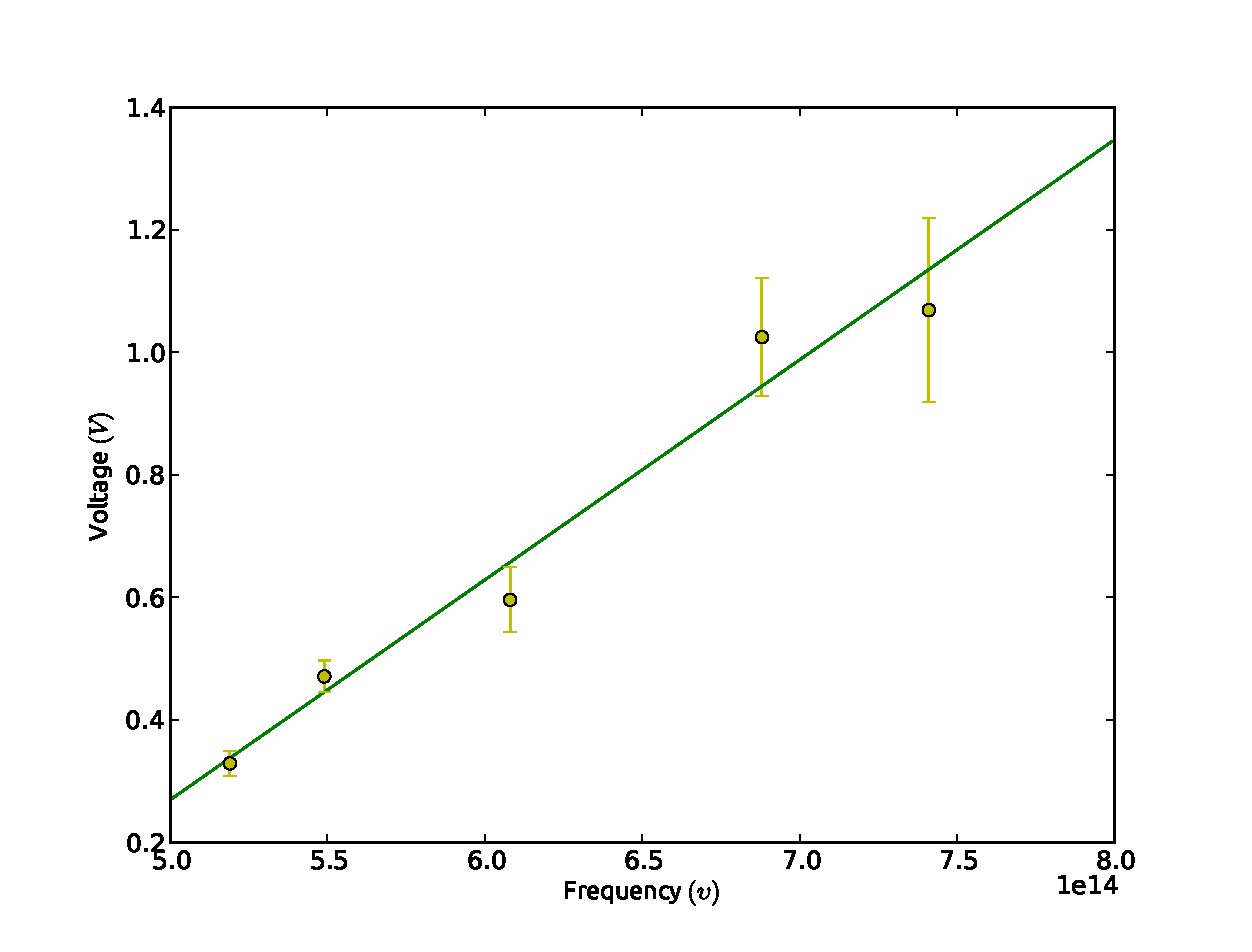
\includegraphics[width=1.0 \columnwidth]{planckconstant.eps}
\end{figure}

This 'Planck's Constant Estimation' plot shows the values:


\begin{table}[ht]
\caption{Planck's Constant and Errors \label{rawdata}}
\centering
\begin{tabular}{cccccc}
\\
 $h$ & $W_0$ & $\sigma_h$ & $\sigma_{W_0}$  \\
\hline
 $5.74x10^{-34}$ & 1.527 & $6.03x10^{-35}$ & 0.205 




  
\end{tabular}
\label{default}
\end{table}





\section{Results}
Our experiment verified our hypothesis. We observed
light behave as if it were a particle (not a wave) in its interaction with matter. We were able to demonstrate for
light the linear dependence of its energy on its wavelength
and determine to some accuracy the constant of proportionality. The actual value of Planck’s constant fell inside of our errorbars, which is more than ideal. Our final
uncertainty on the value proved to be 14.8\% of the value
itself. This is very small and makes the task of drawing
solid conclusions difficult to believe to be close to the real value. 

\begin{center}
$error=\frac{|(6.63-5.74)x10^{-34}|}{6.03x10^{-35}}=14.8\%$
\end{center}


\begin{acknowledgements}
I would like to thank my partner Kadir Simsek  for his help to the experiment, and also to the teaching assistant Saime Sarikaya for her guidance during the experiment.
\end{acknowledgements}

\section{References}
\begin{itemize}
\item 	E. Gulmez, ”Advanced Physics Experiment”, Istanbul, Bogazici University Publication, 1999

\item http://web.mit.edu/8.13/www/experiments.shtml
\end{itemize}

\section{Appendix}


Python code for each color (example belongs to green) $V$ vs. $I$ plot

\begin{lstlisting}

from pylab import *


def VS(m1,n1,m2,n2):
	return abs(n1-n2)/abs(m1-m2)

def sigmavs(m1,n1,m2,n2,sm1,sn1,sm2,sn2):
	return sqrt( (1/(m1-m2))**2*(sn1)**2 + (-1/(m1-m2))**2*(sn2)**2 + ((n2-n1)/(m1-m2)**2)**2*(sm1)**2 +((n1-n2)/(m1-m2))**2*(sm2)**2)



def analysis(x,y):

	sy=ones(len(y))*1e-11
	S   = sum(1 / sy**2)
	Sx  = sum(x / sy**2)
	Sy  = sum(y / sy**2)
	Sxx = sum(x**2 / sy**2)
	Sxy = sum(x*y / sy**2)

	delta = S*Sxx - Sx**2

	n = (Sxx*Sy - Sx*Sxy) / delta
	m = (S*Sxy - Sx*Sy) / delta

	sn = sqrt(Sxx / delta)
	sm = sqrt(S / delta)



	errorbar(x,y,yerr=sy,fmt='o')

	xx = arange(0,1.8,1e-2)
	yy = n + m*xx


	

	return yy,m,n,sm,sn

	


x=[[1.705,0.977,0.565,0.491],[0.405,0.374,0.298]]
y=[[-0.12,-0.10,-0.05,0.0],[0.1,0.15,0.30]]

yy=analysis(array(x[0]),array(y[0])*1e-10)[0]
yy1=analysis(array(x[1]),array(y[1])*1e-10)[0]

m1=analysis(array(x[0]),array(y[0])*1e-10)[1]
n1=analysis(array(x[0]),array(y[0])*1e-10)[2]
sm1=analysis(array(x[0]),array(y[0])*1e-10)[3]
sn1=analysis(array(x[0]),array(y[0])*1e-10)[4]
m2=analysis(array(x[1]),array(y[1])*1e-10)[1]
n2=analysis(array(x[1]),array(y[1])*1e-10)[2]
sm2=analysis(array(x[1]),array(y[1])*1e-10)[3]
sn2=analysis(array(x[1]),array(y[1])*1e-10)[4]

print 'Vs'+str(VS(m1,n1,m2,n2))
print 'Sigma Vs'+str(sigmavs(m1,n1,m2,n2,sm1,sn1,sm2,sn2))

xx=arange(0,1.8,1e-2)

plot(xx,yy)
plot(xx,yy1)
xlabel('Voltage $(V)$',fontname='Ubuntu')
ylabel('Current $(A)$',fontname='Ubuntu')

show()

\end{lstlisting}


Python code for $\upsilon$ vs. $V$ plot:

\begin{lstlisting}
from pylab import *

def analysis(x,y,sy):

	
	S   = sum(1 / sy**2)
	Sx  = sum(x / sy**2)
	Sy  = sum(y / sy**2)
	Sxx = sum(x**2 / sy**2)
	Sxy = sum(x*y / sy**2)

	delta = S*Sxx - Sx**2

	n = (Sxx*Sy - Sx*Sxy) / delta
	m = (S*Sxy - Sx*Sy) / delta

	sn = sqrt(Sxx / delta)
	sm = sqrt(S / delta)



	errorbar(x,y,yerr=sy,fmt='o')

	xx = arange(5e14,8e14,1e12)
	yy = n + m*xx
	

	return yy,m,n,sm,sn


y=array([0.329,0.471,0.596,1.025,1.069])

sy=array([0.020,0.026,0.053,0.096,0.150])*10

x=array([5.19,5.49,6.08,6.88,7.41])*1e14

	
yy=analysis(x,y,sy)[0]

xx = arange(5e14,8e14,1e12)





plot(xx,yy)
xlabel('Frequency $(\upsilon)$',fontname='Ubuntu')
ylabel('Voltage $(V)$',fontname='Ubuntu')


print analysis(x,y,sy)[1]*1.6*1e-19
print analysis(x,y,sy)[2]*(-1)
print analysis(x,y,sy)[3]*1.6*1e-19
print analysis(x,y,sy)[4]




show()


\end{lstlisting}




\end{document}
